\customtitlepage{A Survey on Video Temporal Grounding with Multimodal Large Language Model}{anlong Wu, Wei Liu, Ye Liu, Meng Liu, Liqiang Nie, Zhouchen Lin, and Chang Wen Chen}
\section{A Survey on Video Temporal Grounding with Multimodal Large Language Model}

\subsection{Introduction}
\begin{frame}{Introduction}
    \begin{block}{Abstract}
        With the recent advancements in Multimodal Large Language Models (MLLMs), and proliferation of \textbf{untrimmed video content} on the Internet, \texttt{Video Temporal Grounding} (VTG)
        has emerged as a critical task in the field of \textbf{video understanding} and \textbf{information extraction}.  In this paper, they proposed
        a systematical survey of the current research on \texttt{VTG-MLLMs} through \textbf{three-dimensional taxonomy}:

        \begin{itemize}
            \item \textbf{Functional Roles of MLLMs}: They highlighted their architectural significance
            \item \textbf{Training Paradigms}: They analyzed strategies for \textbf{temporal reasoning} and \textbf{task adoptation}
            \item \textbf{Video Feature Processing}: They discussed \textbf{spatiotemporal representation effectiveness}.
        \end{itemize}
    \end{block}
\end{frame}

\begin{frame}{Introduction}
    \begin{block}{Overview}
        There are many applications of \texttt{VTG-MLLMs}:
        \begin{itemize}
            \item Moment Retrieval
            \item Scene Editing
            \item Video Question Answering
            \item \textbf{Temporal Question Answering}
        \end{itemize}
        Our demand is not only what events occur but also when they \textbf{precisely} happen. And to address this gap, \texttt{Video Temporal Grounding} (VTG) has emerged as a pivotal research area. And it involves \textbf{localizing video segments} that correspond to \textbf{natural language questions}, enabling detailed interaction with video content.
    \end{block}
\end{frame}

\begin{frame}{Introduction}
    \begin{block}{Core Challenge}
        The core challenge of \texttt{VTG} lies in precisely \textbf{aligning complex linguistic semantics} with \texttt{temporal distributed visual information}, while simultaneously handling complex \texttt{temporal relationships} within the video.
    \end{block}
    \begin{block}{Tasks}
        \texttt{VTG} encompasses several distinct tasks:

        \begin{itemize}
            \item \textbf{Video Moment Retrieval (VMR)}: To identify video segments matching NL descriptions.
            \item \textbf{Dense Video Captioning (DVC)}: To generate temporally aligned captions for multiple events.
            \item \textbf{Video Highlight Detection (VHD)}: To select segments most relevant to the query.
            \item \textbf{Temporally Grounded Video Question Answering (TG-VQA)}: To pinpoint the temporal evidence.
        \end{itemize}
    \end{block}
\end{frame}

\begin{frame}{Overview Timeline of Representative VTG-MLLMs}
    \vspace{-0.4em}
    \centering
    \resizebox{\linewidth}{!}{%
    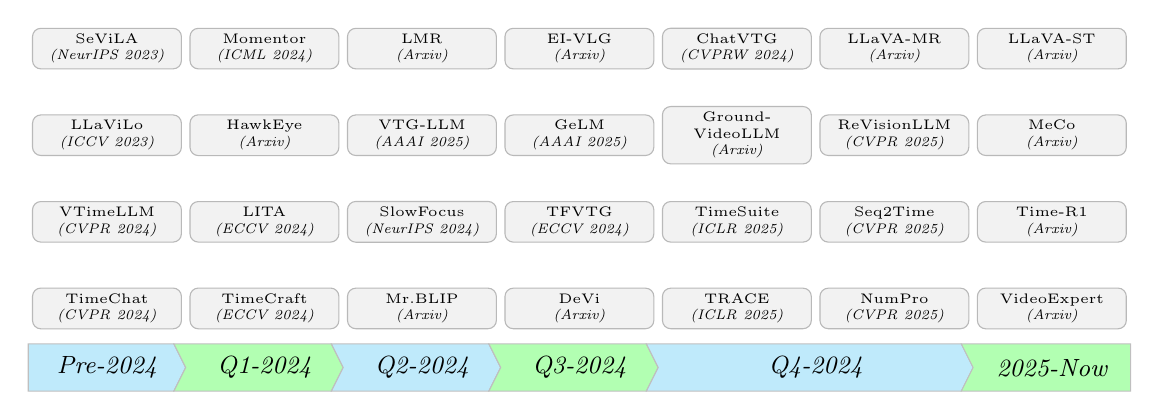
\begin{tikzpicture}

    % Colors: alternating blue/green for time periods
    \colorlet{colorA}{cyan!25}
    \colorlet{colorB}{green!30}

    % Arrow (chevron) height
    \def\ah{0.60}

    % Coordinate layout (1 unit = 1 cm, total width = 14 cm):
    %   6 periods where Q4-2024 is double-wide (2 units × 2 = 4):
    %   Pre-2024 [0,2], Q1-2024 [2,4], Q2-2024 [4,6],
    %   Q3-2024 [6,8], Q4-2024 [8,12], 2025-Now [12,14]
    % Chevron tip offset = 0.15 cm from each boundary

    % Pre-2024  [0, 2]  center=1.0  (flat left, pointed right)
    \filldraw[fill=colorA, draw=gray!50, line width=0.4pt]
        (0,0)--(1.85,0)--(2.0,\ah/2)--(1.85,\ah)--(0,\ah)--cycle;
    \node[font=\small\itshape] at (1.0,\ah/2) {Pre-2024};

    % Q1-2024  [2, 4]  center=3.0
    \filldraw[fill=colorB, draw=gray!50, line width=0.4pt]
        (1.85,0)--(3.85,0)--(4.0,\ah/2)--(3.85,\ah)--(1.85,\ah)--(2.0,\ah/2)--cycle;
    \node[font=\small\itshape] at (3.0,\ah/2) {Q1-2024};

    % Q2-2024  [4, 6]  center=5.0
    \filldraw[fill=colorA, draw=gray!50, line width=0.4pt]
        (3.85,0)--(5.85,0)--(6.0,\ah/2)--(5.85,\ah)--(3.85,\ah)--(4.0,\ah/2)--cycle;
    \node[font=\small\itshape] at (5.0,\ah/2) {Q2-2024};

    % Q3-2024  [6, 8]  center=7.0
    \filldraw[fill=colorB, draw=gray!50, line width=0.4pt]
        (5.85,0)--(7.85,0)--(8.0,\ah/2)--(7.85,\ah)--(5.85,\ah)--(6.0,\ah/2)--cycle;
    \node[font=\small\itshape] at (7.0,\ah/2) {Q3-2024};

    % Q4-2024  [8,12]  center=10.0  (double-wide, 2 sub-columns at x=9 and x=11)
    \filldraw[fill=colorA, draw=gray!50, line width=0.4pt]
        (7.85,0)--(11.85,0)--(12.0,\ah/2)--(11.85,\ah)--(7.85,\ah)--(8.0,\ah/2)--cycle;
    \node[font=\small\itshape] at (10.0,\ah/2) {Q4-2024};

    % 2025-Now [12,14]  center=13.0  (pointed left, flat right)
    \filldraw[fill=colorB, draw=gray!50, line width=0.4pt]
        (11.85,0)--(14.0,0)--(14.0,\ah)--(11.85,\ah)--(12.0,\ah/2)--cycle;
    \node[font=\small\itshape] at (13.0,\ah/2) {2025-Now};

    % Box style: rounded rectangle, consistent width
    \tikzset{mbox/.style={
        draw=gray!55, fill=gray!10, rounded corners=3pt,
        align=center, text width=1.75cm,
        inner xsep=2pt, inner ysep=2pt, font=\tiny
    }}

    % Box row y-positions (4 rows, spacing = 1.1 cm)
    \def\ya{1.05}
    \def\yb{2.15}
    \def\yc{3.25}
    \def\yd{4.35}

    % --- Pre-2024  (x = 1.0) ---
    \node[mbox] at (1.0,\yd) {SeViLA\\\itshape(NeurIPS 2023)};
    \node[mbox] at (1.0,\yc) {LLaViLo\\\itshape(ICCV 2023)};
    \node[mbox] at (1.0,\yb) {VTimeLLM\\\itshape(CVPR 2024)};
    \node[mbox] at (1.0,\ya) {TimeChat\\\itshape(CVPR 2024)};

    % --- Q1-2024  (x = 3.0) ---
    \node[mbox] at (3.0,\yd) {Momentor\\\itshape(ICML 2024)};
    \node[mbox] at (3.0,\yc) {HawkEye\\\itshape(Arxiv)};
    \node[mbox] at (3.0,\yb) {LITA\\\itshape(ECCV 2024)};
    \node[mbox] at (3.0,\ya) {TimeCraft\\\itshape(ECCV 2024)};

    % --- Q2-2024  (x = 5.0) ---
    \node[mbox] at (5.0,\yd) {LMR\\\itshape(Arxiv)};
    \node[mbox] at (5.0,\yc) {VTG-LLM\\\itshape(AAAI 2025)};
    \node[mbox] at (5.0,\yb) {SlowFocus\\\itshape(NeurIPS 2024)};
    \node[mbox] at (5.0,\ya) {Mr.BLIP\\\itshape(Arxiv)};

    % --- Q3-2024  (x = 7.0) ---
    \node[mbox] at (7.0,\yd) {EI-VLG\\\itshape(Arxiv)};
    \node[mbox] at (7.0,\yc) {GeLM\\\itshape(AAAI 2025)};
    \node[mbox] at (7.0,\yb) {TFVTG\\\itshape(ECCV 2024)};
    \node[mbox] at (7.0,\ya) {DeVi\\\itshape(Arxiv)};

    % --- Q4-2024 left sub-column  (x = 9.0) ---
    \node[mbox] at (9.0,\yd) {ChatVTG\\\itshape(CVPRW 2024)};
    \node[mbox] at (9.0,\yc) {Ground-VideoLLM\\\itshape(Arxiv)};
    \node[mbox] at (9.0,\yb) {TimeSuite\\\itshape(ICLR 2025)};
    \node[mbox] at (9.0,\ya) {TRACE\\\itshape(ICLR 2025)};

    % --- Q4-2024 right sub-column  (x = 11.0) ---
    \node[mbox] at (11.0,\yd) {LLaVA-MR\\\itshape(Arxiv)};
    \node[mbox] at (11.0,\yc) {ReVisionLLM\\\itshape(CVPR 2025)};
    \node[mbox] at (11.0,\yb) {Seq2Time\\\itshape(CVPR 2025)};
    \node[mbox] at (11.0,\ya) {NumPro\\\itshape(CVPR 2025)};

    % --- 2025-Now  (x = 13.0) ---
    \node[mbox] at (13.0,\yd) {LLaVA-ST\\\itshape(Arxiv)};
    \node[mbox] at (13.0,\yc) {MeCo\\\itshape(Arxiv)};
    \node[mbox] at (13.0,\yb) {Time-R1\\\itshape(Arxiv)};
    \node[mbox] at (13.0,\ya) {VideoExpert\\\itshape(Arxiv)};

    \end{tikzpicture}
    }
    \vspace{0.2em}
    {\fontsize{6}{7}\selectfont\textit{Fig.~1: An overview timeline of representative VTG-MLLMs, organized by initial arXiv release dates.}}
\end{frame}

\begin{frame}{Introduction}
    \begin{block}{Motivation}
        Motivated by the rapid advancements in \texttt{MLLMs}, unlike traditional approaches relying solely on \textbf{visual backbones} with task-specific heads, \texttt{VTG-MLLMs} utilize \textbf{general-purpose MLLMs} to reason about \textit{temporal relationships, align semantics} and \textit{localize relevant video segments} either directly or indirectly.
    \end{block}
\end{frame}

\subsection{Preliminaries}
\begin{frame}{Video Temporal Grounding}
    \begin{block}{Video Moment Retrieval (VMR)}
        \texttt{VMR} aims to \textbf{identify} and \textbf{localize} temporal segments within untrimmed videos based on NL queries. It not only requires \textbf{accurate alignment} of textual descriptions with specific video segments, but also the \textbf{ability to map} video content to precise \textbf{temporal boundaries}, testing understanding of fine-grained temporal relationships and semantic conherence.
    \end{block}
    \begin{block}{Dense Video Captioning (DVC)}
        \texttt{DVC} involves generating detailed, temporally grounded descriptions for all significant events or actions occuring in a video, along with their corresponding start and end timestamps. Unlike traditional MR, \texttt{DVC} captures the complete narrative by \textbf{identifying multiple events} and their temporal dependencies. It also challenges models to manage \textbf{overlapping events}, a capability essential for achieving comprehensive fine-grained video understanding. 
    \end{block}
\end{frame}

\begin{frame}{Video Temporal Grounding}
    \begin{figure}
        \centering
        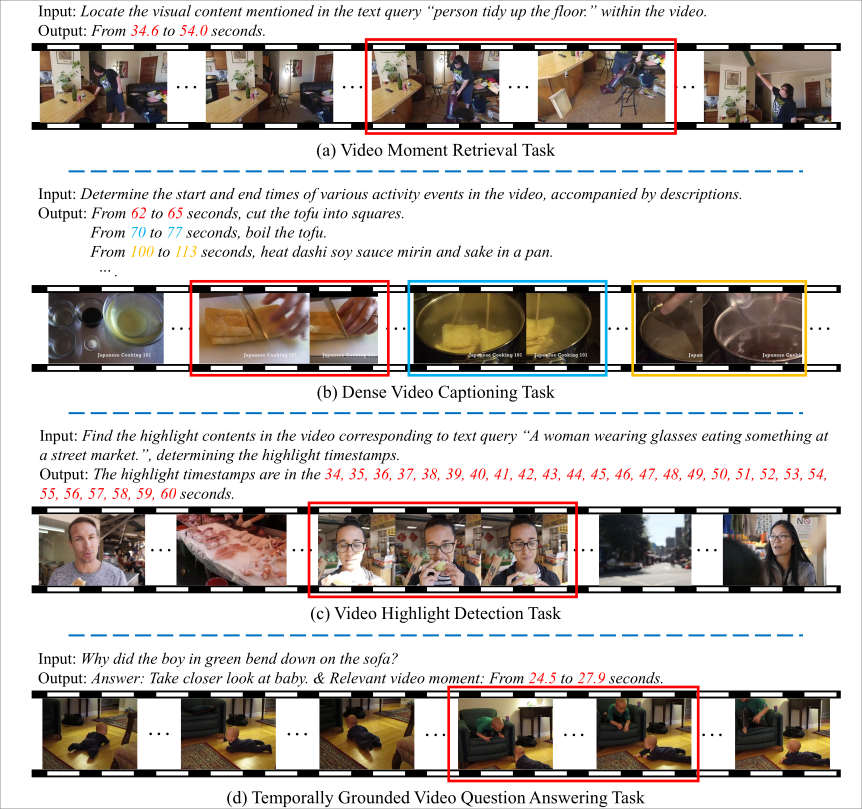
\includegraphics[width=0.5\textwidth]{img/general/ex_vtg.png}
        \caption{An illustration of the Video Temporal Grounding (VTG) task.}
    \end{figure}
\end{frame}

\begin{frame}{Video Temporal Grounding}
    \begin{block}{Video Highlight Detection}
        \texttt{VHD} aims to identify \textbf{keyframes} or \textbf{short segments} within a video that best match a given NL query. Unlike VMR and VDC, it emphasizes \textbf{frame-level precision} and evalute the ability of model to accurately pinpoint salient video clips that closely correspond to prompts and to access their contextual significance.  
    \end{block}

    \begin{block}{Temporally Grounded Video Question Answering (TG-VQA)}
        \texttt{TG-VQA} requires models to not only provide answer questions bu also identify and localize the precise temporal intervals containing relevant visual evidence. It introduces the added complexity of integrating temporal localization with multimodal reasoning.
    \end{block}
\end{frame}

\subsection{A Multi-Faceted Taxonomy of VTG-MLLMs}
% ── Slide 3.1 ────────────────────────────────────────────────────────────────
\begin{frame}{Section 3.1 -- Functional Roles of MLLMs}
\vspace{-0.5em}
\centering
\resizebox{\linewidth}{!}{%
\begin{tikzpicture}[
    root/.style={draw=gray!70,fill=gray!25,rounded corners=4pt,align=center,
                 font=\normalsize\bfseries,inner sep=5pt},
    sec/.style={draw=UFTblue!80,fill=UFTblue!20,rounded corners=4pt,align=center,
                font=\small\bfseries,inner sep=5pt,text width=2.4cm},
    cat/.style={draw=orange!80,fill=orange!18,rounded corners=4pt,align=center,
                font=\small\bfseries,inner sep=4pt,minimum width=2.4cm},
    mlist/.style={draw=PROFMATgreen!65,fill=PROFMATgreen!10,rounded corners=4pt,
                  align=left,font=\tiny,inner sep=5pt,text width=6.2cm}
]

\node[root] (vtg) {VTG-\\MLLMs};
\node[sec,right=0.5cm of vtg] (sec) {Section 3.1\\Functional\\Roles of MLLMs};
\draw[gray!60,line width=0.6pt] (vtg.east)--(sec.west);

\coordinate (bp) at ($(sec.east)+(0.4,0)$);
\draw[gray!60] (sec.east)--(bp);
\draw[gray!60] ($(bp)+(0,-2.2)$)--($(bp)+(0,1.9)$);

\node[cat] (fac) at ($(bp)+(1.9, 1.9)$) {Facilitator};
\node[cat] (exe) at ($(bp)+(1.9,-2.2)$) {Executor};
\draw[gray!60] ($(bp)+(0, 1.9)$)--(fac.west);
\draw[gray!60] ($(bp)+(0,-2.2)$)--(exe.west);

\node[mlist,right=0.3cm of fac] (facm) {%
  ChatVTG [29], TEA [91], TimeCraft [56], GroundVQA [91], TFVTG [92],
  Grounding-Prompter [93], VTG-GPT [94], VERIFIED [95], EI-VLG [96],
  VideoLights [97], GPTSee [98], LMR [99], ReCorrect [100], DeVi [32], Moment-GPT [101]%
};
\draw[gray!60] (fac.east)--(facm.west);

\node[mlist,right=0.3cm of exe] (exem) {%
  SeViLA [102], LLaViLo [103], TimeChat [27], MLLM-TA [104], LITA [111],
  TemporalVLM [118], NumPro [106], TRACE [31], VTimeLLM [26], Seq2Time [107],
  Grounded-VideoLLM [54], TimeSuite [33], VTG-LLM [108], GroundingGPT [109],
  ReVisionLLM [110], GeLM [115], TimeRefine [112], TimeMarker [114], Momentor [28],
  SlowFocus [116], LLaVA-ST [113], TPE-VLLM [120], E.T.Chat [51], MeCo [123],
  VideoMind [35], SpaceVLLM [122], VideoExpert [124], Time-R1 [124],
  VideoChat-R1 [126], MUSEG [127]%
};
\draw[gray!60] (exe.east)--(exem.west);

\end{tikzpicture}
}
\end{frame}

% ── Slide 3.2 ────────────────────────────────────────────────────────────────
\begin{frame}{Section 3.2 -- Training Paradigms}
\vspace{-0.5em}
\centering
\resizebox{\linewidth}{!}{%
\begin{tikzpicture}[
    root/.style={draw=gray!70,fill=gray!25,rounded corners=4pt,align=center,
                 font=\normalsize\bfseries,inner sep=5pt},
    sec/.style={draw=UFTblue!80,fill=UFTblue!20,rounded corners=4pt,align=center,
                font=\small\bfseries,inner sep=5pt,text width=2.4cm},
    cat/.style={draw=orange!80,fill=orange!18,rounded corners=4pt,align=center,
                font=\small\bfseries,inner sep=4pt,minimum width=2.4cm},
    mlist/.style={draw=PROFMATgreen!65,fill=PROFMATgreen!10,rounded corners=4pt,
                  align=left,font=\tiny,inner sep=5pt,text width=6.2cm}
]

\node[root] (vtg) {VTG-\\MLLMs};
\node[sec,right=0.5cm of vtg] (sec) {Section 3.2\\Training\\Paradigms};
\draw[gray!60,line width=0.6pt] (vtg.east)--(sec.west);

\coordinate (bp) at ($(sec.east)+(0.4,0)$);
\draw[gray!60] (sec.east)--(bp);
\draw[gray!60] ($(bp)+(0,-2.6)$)--($(bp)+(0,2.6)$);

\node[cat] (pre) at ($(bp)+(1.9, 2.6)$) {Pretraining};
\node[cat] (ft)  at ($(bp)+(1.9, 0.0)$) {Fine-Tuning};
\node[cat] (tf)  at ($(bp)+(1.9,-2.6)$) {Training-Free};
\draw[gray!60] ($(bp)+(0, 2.6)$)--(pre.west);
\draw[gray!60] ($(bp)+(0, 0.0)$)--(ft.west);
\draw[gray!60] ($(bp)+(0,-2.6)$)--(tf.west);

\node[mlist,right=0.3cm of pre] (prem) {%
  SeViLA [102], VTimeLLM [26], TimeChat [27], VTG-LLM [108], TemporalVLM [118],
  Seq2Time [107], VideoChat-TPO [121], Grounded-VideoLLM [54], HawkEye [32],
  TRACE [31], TimeRefine [112], TimeMarker [114], Momentor [28],
  ReVisionLLM [110], SlowFocus [116], LLaVA-ST [113], MeCo [123],
  Time-R1 [124], VideoChat-R1 [126], MUSEG [127]%
};
\draw[gray!60] (pre.east)--(prem.west);

\node[mlist,right=0.3cm of ft] (ftm) {%
  LLaViLo [103], Mr.BLIP [117], LLaVA-MR [105], VideoLights [97],
  TGB [119], GPTSee [98], EI-VLG [96], LMR [99], TEA [90], ReCorrect [100]%
};
\draw[gray!60] (ft.east)--(ftm.west);

\node[mlist,right=0.3cm of tf] (tfm) {%
  NumPro [106], ChatVTG [29], DeVi [32], TFVTG [92],
  VTG-GPT [94], Moment-GPT [103], Grounding-Prompter [95]%
};
\draw[gray!60] (tf.east)--(tfm.west);

\end{tikzpicture}
}
\end{frame}

% ── Slide 3.3 ────────────────────────────────────────────────────────────────
\begin{frame}{Section 3.3 -- Feature Processing Techniques}
\vspace{-0.5em}
\centering
\resizebox{\linewidth}{!}{%
\begin{tikzpicture}[
    root/.style={draw=gray!70,fill=gray!25,rounded corners=4pt,align=center,
                 font=\normalsize\bfseries,inner sep=5pt},
    sec/.style={draw=UFTblue!80,fill=UFTblue!20,rounded corners=4pt,align=center,
                font=\small\bfseries,inner sep=5pt,text width=2.4cm},
    cat/.style={draw=orange!80,fill=orange!18,rounded corners=4pt,align=center,
                font=\small\bfseries,inner sep=4pt,text width=2.2cm},
    subcat/.style={draw=orange!60,fill=orange!10,rounded corners=3pt,align=center,
                   font=\scriptsize\bfseries,inner sep=3pt,minimum width=2.4cm},
    mlist/.style={draw=PROFMATgreen!65,fill=PROFMATgreen!10,rounded corners=4pt,
                  align=left,font=\tiny,inner sep=5pt,text width=3.8cm}
]

\node[root] (vtg) {VTG-\\MLLMs};
\node[sec,right=0.5cm of vtg] (sec) {Section 3.3\\Feature Processing\\Techniques};
\draw[gray!60,line width=0.6pt] (vtg.east)--(sec.west);

% Main spine
\coordinate (bp) at ($(sec.east)+(0.4,0)$);
\draw[gray!60] (sec.east)--(bp);
\draw[gray!60] ($(bp)+(0,-1.5)$)--($(bp)+(0,1.5)$);

% Level-1 category nodes
\node[cat] (vis) at ($(bp)+(1.8, 1.5)$) {Visual\\Feature};
\node[cat] (tem) at ($(bp)+(1.8,-1.5)$) {Temporal\\Feature};
\draw[gray!60] ($(bp)+(0, 1.5)$)--(vis.west);
\draw[gray!60] ($(bp)+(0,-1.5)$)--(tem.west);

% Visual sub-spine  (comp above, refi below vis)
\coordinate (vbp) at ($(vis.east)+(0.4,0)$);
\draw[gray!60] (vis.east)--(vbp);
\draw[gray!60] ($(vbp)+(0,-0.8)$)--($(vbp)+(0,0.8)$);

\node[subcat] (comp) at ($(vbp)+(1.5, 0.8)$) {With\\Compression};
\node[subcat] (refi) at ($(vbp)+(1.5,-0.8)$) {With\\Refinement};
\draw[gray!60] ($(vbp)+(0, 0.8)$)--(comp.west);
\draw[gray!60] ($(vbp)+(0,-0.8)$)--(refi.west);

% Temporal sub-spine  (expl above, impl below tem)
\coordinate (tbp) at ($(tem.east)+(0.4,0)$);
\draw[gray!60] (tem.east)--(tbp);
\draw[gray!60] ($(tbp)+(0,-0.8)$)--($(tbp)+(0,0.8)$);

\node[subcat] (expl) at ($(tbp)+(1.5, 0.8)$) {Explicit};
\node[subcat] (impl) at ($(tbp)+(1.5,-0.8)$) {Implicit};
\draw[gray!60] ($(tbp)+(0, 0.8)$)--(expl.west);
\draw[gray!60] ($(tbp)+(0,-0.8)$)--(impl.west);

% Model lists
\node[mlist,right=0.3cm of comp] (compm) {%
  ReVisionLLM [110], LLaVA-MR [105], E.T.Chat [51], VTG-LLM [108],
  LITA [111], Grounded-VideoLLM [54], TRACE [31], TimeMarker [114],
  LLaVA-ST [113], TimeSuite [33], VideoExpert [125]%
};
\draw[gray!60] (comp.east)--(compm.west);

\node[mlist,right=0.3cm of refi] (refim) {%
  SeViLA [102], HawkEye [32], VideoMind [35],
  SlowFocus [116], ReVisionLLM [110]%
};
\draw[gray!60] (refi.east)--(refim.west);

\node[mlist,right=0.3cm of expl] (explm) {%
  LLaVA-MR [105], TRACE [31], LITA [111], VTG-LLM [108],
  Mr.BLIP [117], Momentor [28], TimeMarker [114],
  LLaVA-ST [113], TGB [119], VideoExpert [125]%
};
\draw[gray!60] (expl.east)--(explm.west);

\node[mlist,right=0.3cm of impl] (implm) {%
  NumPro [106], HawkEye [32], ReVisionLLM [110], GroundingGPT [109],
  TimeRefine [112], VTimeLLM [26], TimeChat [27],
  Grounded-VideoLLM [54], TemporalVLM [118], TimeSuite [33], VideoMind [35]%
};
\draw[gray!60] (impl.east)--(implm.west);

\end{tikzpicture}
}
\end{frame}

\subsection{Directions}
\begin{frame}{Directions}
    \begin{block}{Four Directions}
        \begin{itemize}
            \item \textbf{Video Temporal Grounding}: to locate specific moments in a video based on a text query. 
            \item \textbf{Video Highlighting Detection}: to identify engagin segments within a given video, which requires to assign a saliency score to each video clip and select the highest-scoring.
            \item \textbf{Dense Video Captioning}: Requires both \textit{event localization} and \textit{captioning} within the same framework.
            \item \textbf{Video Grounding Question Answering}: Requires models to understand video content to answer questions and to locate relevant segments as visual evidence.
        \end{itemize}
    \end{block}
\end{frame}